\documentclass[12pt]{article}
\usepackage{fullpage}
\usepackage[utf8]{inputenc}
\usepackage{pict2e}
\usepackage{amsmath}
\usepackage{enumitem}
\usepackage{eurosym}
\usepackage{mathtools}
\usepackage{amssymb, amsfonts, latexsym, cancel}
\setlength{\parskip}{0.3cm}
\usepackage{graphicx}
\usepackage{fontenc}
\usepackage{slashbox}
\usepackage{setspace}
\usepackage{gensymb}
\usepackage{accents}
\usepackage{adjustbox}
\setstretch{1.35}
\usepackage{bold-extra}
\usepackage{subcaption}
\usepackage{tcolorbox}
\usepackage{xcolor, colortbl}
\usepackage{wrapfig}
\usepackage{empheq}
\usepackage{array}
\usepackage{parskip}
\usepackage{arydshln}
\graphicspath{ {images/} }
\renewcommand*\contentsname{\color{black}Índice} 
\usepackage{array, multirow, multicol}
\definecolor{lightblue}{HTML}{007AFF}
\usepackage{color}
\usepackage{etoolbox}
\usepackage{listings}
\usepackage{mdframed}
\setlength{\parindent}{0pt}
\usepackage{underscore}
\usepackage{hyperref}
\usepackage{tikz}
\usepackage{tikz-cd}
\usetikzlibrary{shapes, positioning, patterns}
\usepackage{tikz-qtree}
\usepackage{biblatex}
\usepackage{pdfpages}
\usepackage{pgfplots}
\usepackage{pgfkeys}
\addbibresource{biblatex-examples.bib}
\usepackage[a4paper, left=1cm, right=1cm, top=1cm, bottom=1.5cm]{geometry}
\usepackage{titlesec}
\usepackage{titletoc}
\usepackage{tikz-3dplot}
\usepackage{kbordermatrix}
\usetikzlibrary{decorations.pathreplacing}
\newcommand{\Ej}{\textcolor{lightblue}{\underline{Ejemplo}}}
\setlength{\fboxrule}{1.5pt}

\newcommand{\bboxed}[1]{\fcolorbox{lightblue}{lightblue!10}{$#1$}}
\newcommand{\rboxed}[1]{\fcolorbox{red}{red!10}{$#1$}}

\DeclareMathOperator{\N}{\mathbb{N}}
\DeclareMathOperator{\Z}{\mathbb{Z}}
\DeclareMathOperator{\R}{\mathbb{R}}
\DeclareMathOperator{\Q}{\mathbb{Q}}
\DeclareMathOperator{\K}{\mathbb{K}}
\DeclareMathOperator{\im}{\imath}
\DeclareMathOperator{\jm}{\jmath}
\DeclareMathOperator{\col}{\mathrm{Col}}
\DeclareMathOperator{\fil}{\mathrm{Fil}}
\DeclareMathOperator{\rg}{\mathrm{rg}}
\DeclareMathOperator{\nuc}{\mathrm{nuc}}
\DeclareMathOperator{\dimf}{\mathrm{dimFil}}
\DeclareMathOperator{\dimc}{\mathrm{dimCol}}
\DeclareMathOperator{\dimn}{\mathrm{dimnuc}}
\DeclareMathOperator{\dimr}{\mathrm{dimrg}}
\DeclareMathOperator{\dom}{\mathrm{Dom}}
\DeclareMathOperator{\infi}{\int_{-\infty}^{+\infty}}
\newcommand{\dint}[2]{\int_{#1}^{#2}}

\newcommand{\bu}[1]{\textcolor{lightblue}{\underline{#1}}}
\newcommand{\lb}[1]{\textcolor{lightblue}{#1}}
\newcommand{\db}[1]{\textcolor{blue}{#1}}
\newcommand{\rc}[1]{\textcolor{red}{#1}}

\renewcommand{\CancelColor}{\color{lightblue}}
\newcommand{\code}[1]{\texttt{\textbf{#1}}}

\usepackage{textgreek}

\newcommand{\dx}{\:\mathrm{d}x}
\newcommand{\dt}{\:\mathrm{d}t}
\newcommand{\dy}{\:\mathrm{d}y}
\newcommand{\dz}{\:\mathrm{d}z}
\newcommand{\dth}{\:\mathrm{d}\theta}
\newcommand{\dr}{\:\mathrm{d}\rho}
\newcommand{\du}{\:\mathrm{d}u}
\newcommand{\dv}{\:\mathrm{d}v}
\newcommand{\tozero}[1]{\cancelto{0}{#1}}
\newcommand{\lbb}[2]{\textcolor{lightblue}{\underbracket[1pt]{\textcolor{black}{#1}}_{#2}}}
\newcommand{\dbb}[2]{\textcolor{blue}{\underbracket[1pt]{\textcolor{black}{#1}}_{#2}}}
\newcommand{\rub}[2]{\textcolor{red}{\underbracket[1pt]{\textcolor{black}{#1}}_{#2}}}

\titleformat{\section}{\normalfont\LARGE\bfseries}{\thesection.}{10 pt}{}

\title{\textbf{\huge Práctica 2 de Señales y Sistemas}\\ Convolución y análisis de sistemas LTI}
\author{Francisco Javier Mercader Martínez\\ Rubén Gil Martínez}
\date{}

\usepackage{matlab-prettifier}

\lstset{
	language=matlab,
	basicstyle=\ttfamily\small,
	keywordstyle=\color{blue},
	commentstyle=\color{green!70!black},
	stringstyle=\color{red},
	showstringspaces=false,
	breaklines=true,
	frame=single,
	backgroundcolor=\color{lightgray!10},
	captionpos=b,
	tabsize=2,
	inputencoding=utf8,
	literate={á}{{\'a}}1 {é}{{\'e}}1 {í}{{\'i}}1 {ó}{{\'o}}1 {ú}{{\'u}}1{ñ}{{\~n}}1
}

\begin{document}
	\maketitle
	\newpage
	\section{Convolución de señales discretas}
La convolución de dos señales discretas viene dada por la expresión \[ y[n]=h[n]\cdot x[n]=\sum_{k=-\infty}^{\infty}x[k]h[n-k] \]La convolución de dos señales se puede entender de dos maneras desde el punto de vista analítico:
\begin{enumerate}[label=\arabic*)]
	\item En la primera a cada impulso de la señal de entrada, el sistema responde con la respuesta al impulso ponderada por el valor de la señal en ese momento, así: \[ y[n]=\cdots+x[-1]h[n+1]+x[0]h[n]+x[1]h[n-1]+x[2]h[n-2]+\cdots \]
	\item Para la segunda en cada instante de tiempo discreto $n$ la señal de salida $y[n]$ se calcula asumiendo que el eje de tiempos es $k$, se queda fija la señal de entrada, y se invierte y  se desplaza a $n$ la respuesta al impulso, multiplicándose finalmente ambas señales y sumando todos sus valores. De esta manera podemos obtener el resultado:
	\[ \begin{array}{l}
		\cdots\\
		y[-1]=\sum_{k=-\infty}^{\infty}x[k]h[-1-k]\\
		y[0]=\sum_{k=-\infty}^{\infty}x[k]h[0-k]\\
		y[1]=\sum_{k=-\infty}^{\infty}x[k]h[1-k]\\
		\cdots
	\end{array} \]
\end{enumerate}
\subsection*{Cuestiones}
\begin{itemize}[leftmargin=*]
	\item \textbf{Calcule previamente de manera gráfica y a mano la convolución de las dos señales casuales $\mathbf{x[n]}$ y $\mathbf{h[n]}$} que definiremos en MATLAB de la siguiente manera.
	\begin{itemize}[label=\textbullet]
		\item \code{x = [1 2 -2];}
		\item \code{h = [1 3 0 1 2 1 2];}
	\end{itemize}
	
\begin{lstlisting}
x = [1 2 -2];
h = [1 3 0 1 2 1 2];

y = conv(x, h);
\end{lstlisting}

\begin{center}
	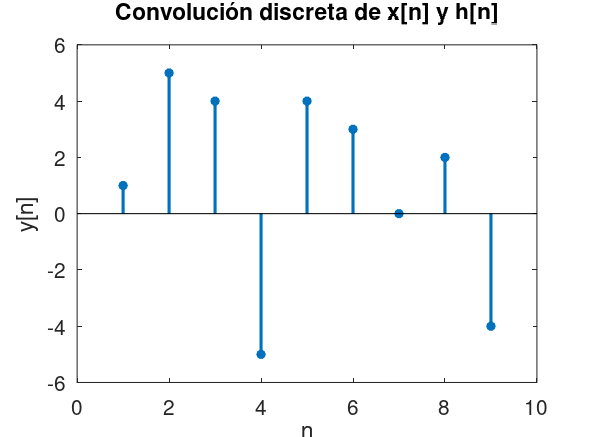
\includegraphics[width=0.7\linewidth]{Imágenes/Figura1}
\end{center}

	\item \textbf{Teniendo en cuneta que la longitud de la secuencia $\mathbf{x[n]}$ es $\mathbf{N}$ y la de $\mathbf{h[n]}$ es $\mathbf{M}$, deduzca una expresión para la longitud de $\mathbf{y[n]}$.}
	
	\begin{lstlisting}
longitud_y = length(x) + length(h) - 1;  % = 9
	\end{lstlisting}
	
	\item Programa dos funciones MATLAB, denominadas \code{conv1} y \code{conv2}, que implementen la convolución de dos señales dsicretas mediante el método 1 y el método 2, explicados anteriormente. Las funciones tendrán el formato \code{y=conv1(x,h)} y \code{y=conv2(x,h)}. Puede inicializar la longitud de la señal de salida deducida en el punto anterior al implementear las funciones. Proporcione el código desarrollado.
	
\begin{lstlisting}[language=matlab]
function y = conv1(x, h)
	% N es la longitud de la secuencia x
	N = length(x);
	% M es la longitud de la secuencia h
	M = length(h);
	% Inicializa la secuencia de salida y con ceros
	y = zeros(1, N+M-1);
	% Itera sobre cada elemento de la secuencia de salida
	for n = 1:N+M-1
		% Itera sobre los elementos de x y h que se superponen para el elemento actual de y
		for k = max(1, n+1-M):min(n, N)
			% Suma el producto de los elementos correspondientes de x y h a la secuencia de salida
			y(n) = y(n) + x(k) * h(n-k+1);
		end
	end
end

function y = conv2d(x, h)
	% Obtén las dimensiones de las matrices de entrada
	[xRows, xCols] = size(x);
	[hRows, hCols] = size(h);
	% Inicializa la matriz de salida
	y = zeros(xRows + hRows - 1, xCols + hCols - 1);
	% Realiza la convolución
	for i = 1:xRows
		for j = 1:xCols
			for m = 1:hRows
				for n = 1:hCols
					y(i+m-1, j+n-1) = y(i+m-1, j+n-1) + x(i, j) * h(m, n);
				end
			end
		end
	end
end

% El objetivo de los bucles es que simulen un sumatorio que mantenga la
% señal "x" fija y que la señal de respuesta al impulso se vaya desplazando
% (iterando) para así ir actualizando los valores de la señal "y"
\end{lstlisting}
	
	\begin{lstlisting}[language=matlab]
y1 = conv1(x,h);

figure(2)
stem(y1, "filled", "LineWidth", 1.5, "MarkerSize", 4);
xlabel('n');
ylabel("y[n]")
title('Conv1 y[n]')
	\end{lstlisting}
	\begin{center}
		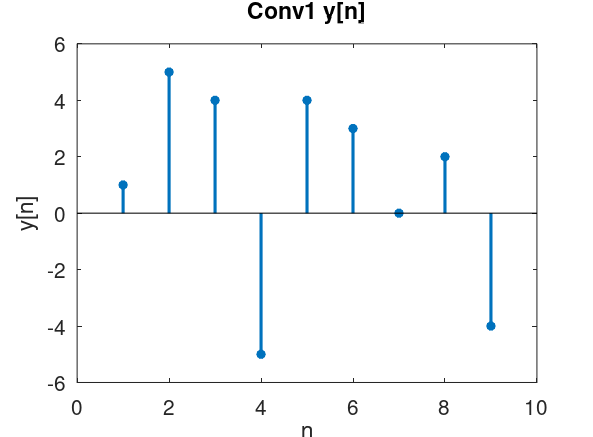
\includegraphics[width=0.7\linewidth]{Imágenes/Figura2}
	\end{center}
\begin{lstlisting}[language=matlab]
y2 = conv2d(x, h);

figure(3)
stem(y2, "filled", "LineWidth", 1.5, "MarkerSize", 4);
xlabel('n');
ylabel("y[n]")
title('Conv2 y[n]')
\end{lstlisting}
	\begin{center}
		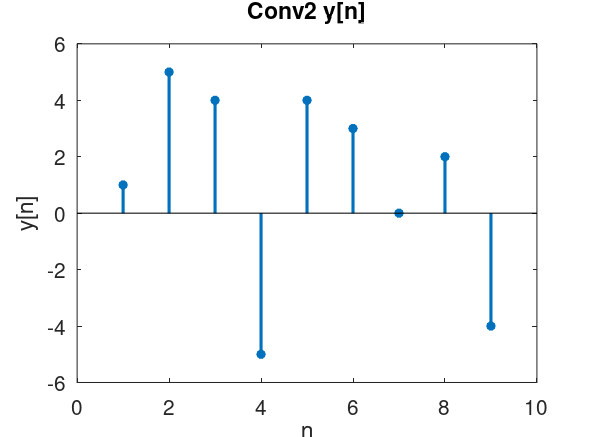
\includegraphics[width=0.7\linewidth]{Imágenes/Figura3}
	\end{center}
	\item Compruebe el correcto funcionamiento de las funciones empleando las señales $x[n]$ y $h[n]$ generadas en MATLAB previamente. Consulta la ayuda (con el comnado \code{help}) de la función \code{conv} de MATLAB, que implementa la convolución discreta de dos secuencias. El resultado con \code{conv}, \code{conv1} y \code{conv2} ha de ser el mismo con cualquier par de señales de entrada.
	
\begin{lstlisting}[language=matlab]
% Las siguientes funciones recorren todos los elementos de las señales y
% comprueban si sus valores coinciden con valores binarios (1 sí, 0 no).
disp(all(y == y1)); % 1
disp(all(y == y2)); % 1
disp(all(y1 == y2)); % 1
\end{lstlisting}
\end{itemize}
\section{Respuesta al impulso de un sistema lineal}
La respuesta al impulso $h[n]$ se emplea para caracterizar el comportamiento de un sistema lineal e invariante (LTI – Linear Time-Invariant). Podremos clasificar el comportamiento de los sistemas LTI atendiendo a la duración finita o infinita de la respuesta al impulso. Por lo tanto, hablaremos respectivamente de sistemas FIR (Finite Impulse Response) o bien de sistemas IIR (Infinite Impulse Response).
\subsection*{Cuestiones}
\subsubsection*{Sistemas FIR}
\[ y[n]=2x[n]+x[n-1]-2x[n-2]+x[n-3] \]
\begin{itemize}
	\item \textbf{Como estudio previo represente el diagrama de bloques (con delays, multiplicadores y sumadores) que caracteriza a este sistema.}
	
	\begin{center}
		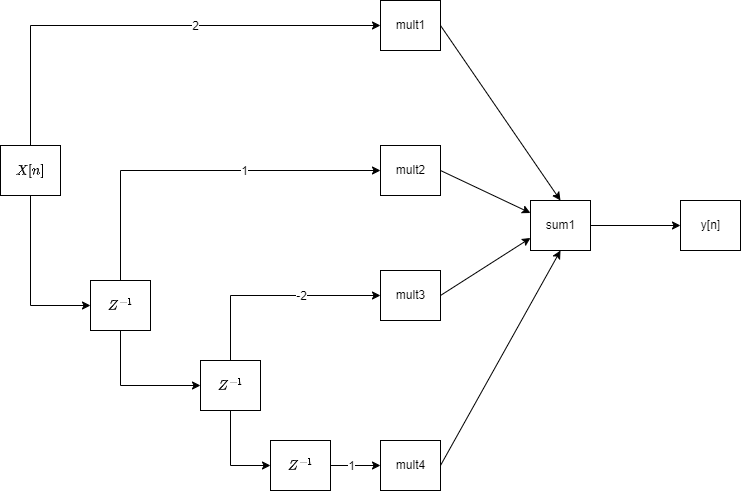
\includegraphics[width=\linewidth]{Imágenes/screenshoot001.drawio}
	\end{center}
	
	\item \textbf{Como estudio previo calcule y represente gráficamente a mano la respuesta al impulso $h[n]$ del sistema dado. ¿Es de duración finita?}
	
	\begin{tikzpicture}[scale=1.5]
		\draw[->] (-2.5,0) -- (6.5,0) node[right] {$n$};
		\draw[->] (0,-2.5) -- (0,2.5) node[above] {$h[n]$};
		
		% Add your impulse response values here
		\foreach \x/\y in {-2/0, -1/0, 0/2, 1/1, 2/-2, 3/1, 4/0, 5/0, 6/0}
		{\draw[fill, lightblue] (\x,\y) circle [radius=0.1];
		\draw[lightblue, line width=2] (\x,0) -- (\x,\y);};
	\end{tikzpicture}
	
	La respuesta al impulso se obtiene al aplicar un impulso unitario (delta de Dirac) a la entrada del sistema. En este caso, si $x[n] = \delta[n]$, entonces:
	
	\code{h[n]=2*\textdelta[n] - \textdelta[n-1] - 2*\textdelta[n-2] + \textdelta[n-3]}
	
	Por lo tanto, la respuesta al impulso es de duración finita y se extiende desde n=0 hasta n=3.
	\item \textbf{Como estudio calcule a mano la salida del sistema ante la entrada $\mathbf{x[n]=\delta[n]-\delta[n-1]}$}, (en MATLAB \code{x=[1 -1]}).
	
	Para calcular la salida del sistema ante la entrada dada, habrá que sustituir \code{x[n]} en la ecución \code{y[n]} con los valores de \code{x[n]} que se han proporcionado.
	
	La entrada es \code{x[n]=\textdelta[n]-\textdelta[n-1]}, que en términos de una secuencia de valores es \code{x[n] = [1 -1]}. Esto significa que \code{x[0] = 1, x[1] = -1} y \code{x[n] = 0} para \code{n < 0} y \code{n > 1}.
\end{itemize}
Calcule la salida con la función \code{conv} (o \code{convol1}, \code{convol2}) en Matlab y verifique que los
resultados coinciden con el estudio \textbf{previo}

\begin{lstlisting}
x = [1 -1];
h = [2 1 -2 1];

% Calcular la secuencia de y[n] mediante la convolución de x[n] y h[n]
y = conv(x, h);
y1 = conv1(x, h);
y2 = conv2d(x, h);

disp(y) % [2 -1 -3 3 -1]
disp(y1) % [2 -1 -3 3 -1]
disp(y2) % [2 -1 -3 3 -1]
\end{lstlisting}
\subsubsection*{Sistemas IIR}
Para un sistema IIR causal definido por la ecuación en diferencias \[ y[n]-\dfrac{4}{5}y[n-1]=x[n] \]
Teniendo en cuenta que se trata de un sistema IIR la respuesta al impulso es de duración infinita. Dado que $h[n]$ es la duración infinita no se podrá emplear la función \code{conv} de MATLAB para obtener exactamente la salida de este sistema ante cualquier señal de entrada. Para estos casos, MATLAB ofrece la función \code{filter} con la que podemos calcular la salida del sistema a partir de la entrada y la ecuación en diferencias.
\begin{itemize}
	\item \textbf{Como estudio previo calcule analíticamente la respuesta al impulso del sistema anterior.} Genere en MATLAB la respuesta al impulso mediante la función \code{filter} y tomando $x[n]$ como \linebreak \code{x=[1 zeros(1, 24)]}. Verifique que el resultado teórico y el práctico coinciden.
	
	\begin{lstlisting}
b = [1]; % Coefifientes de x[n]
a = [1 -4/5]; % Coefifientes de y[n]

% Definir la entrada como un impulso
x = [1 zeros(1, 24)];

% Calcular la respuesta al impulso
h = filter(b, a, x)

disp(h)
	\end{lstlisting}
	
\begin{verbatim}
h =
1.0000e+00  8.0000e-01  6.4000e-01  5.1200e-01  4.0960e-01  3.2768e-01  2.6214e-01
2.0972e-01  1.6777e-01  1.3422e-01  1.0737e-01  8.5899e-02  6.8719e-02  5.4976e-02
4.3980e-02  3.5184e-02  2.8147e-02  2.2518e-02  1.8014e-02  1.4412e-02  1.1529e-02
9.2234e-03  7.3787e-03  5.9030e-03  4.7224e-03
\end{verbatim}

\begin{lstlisting}
% Representación gráfica
figure(4)
stem(n=[0:24], h, "filled", "LineWidth", 1.5, "MarkerSize", 4);
xlabel("n");
title("h[n]")
\end{lstlisting}

\begin{center}
	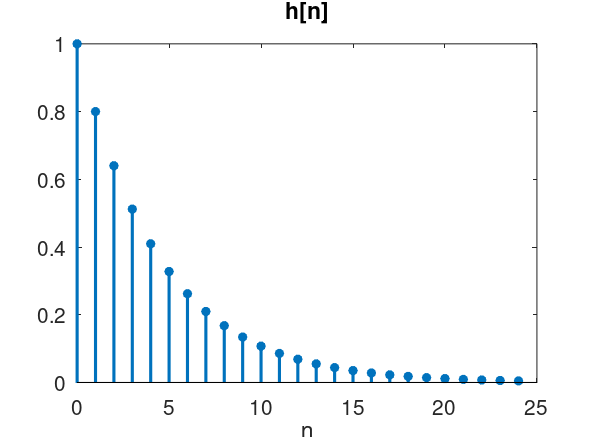
\includegraphics[width=0.7\linewidth]{Imágenes/Figura4}
\end{center}
	
	\item \textbf{Como estudio previo calcule analíticamente la respuesta del sistema ante la siguiente señal de entrada:} \[ x[n]=\left(\dfrac{1}{3}\right)^nu[n] \] Genere en MATLAB la señal $x[n]$ en el intervalo [0:49]. Genere en MATLAB la salida del sistema ante la entrada $x[n]$ empleando de nuevo la función \code{filter}. Compruebe que el resultado práctico coincide con la solución teórica.
	
	\begin{lstlisting}
% Generar la señal de entrada
n = 0:49;
x = (1/3).^n;

% Calcular la respuesta del sistema
y = filter(b, a, x);
	\end{lstlisting}
	
\begin{verbatim}
y = 
1.0000e+00  1.1333e+00  1.0178e+00  8.5126e-01  6.9335e-01  5.5880e-01  4.4841e-01
3.5919e-01  2.8750e-01  2.3005e-01  1.8406e-01  1.4725e-01  1.1780e-01  9.4243e-02  
7.5395e-02  6.0316e-02  4.8253e-02  3.8602e-02  3.0882e-02  2.4705e-02  1.9764e-02  
1.5811e-02  1.2649e-02  1.0119e-02  8.0955e-03  6.4764e-03  5.1811e-03  4.1449e-03  
3.3159e-03  2.6527e-03  2.1222e-03  1.6977e-03  1.3582e-03  1.0866e-03  8.6925e-04  
6.9540e-04  5.5632e-04  4.4505e-04  3.5604e-04  2.8483e-04  2.2787e-04  1.8229e-04  
1.4584e-04  1.1667e-04  9.3335e-05  7.4668e-05  5.9734e-05  4.7787e-05  3.8230e-05  
3.0584e-05
\end{verbatim}
\pagebreak
\begin{lstlisting}
% Representación gráfica
figure(5)
stem(n, y, "filled", "LineWidth", 1.5, "MarkerSize", 4);
xlabel("n");
title("y[n]")
\end{lstlisting}
\begin{center}
	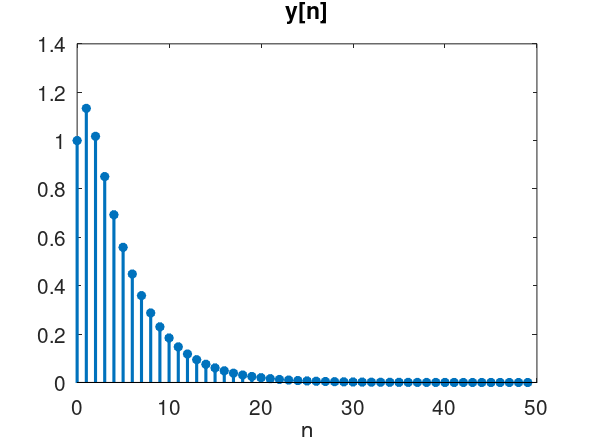
\includegraphics[width=0.7\linewidth]{Imágenes/Figura5}
\end{center}
	
	\item Repita el proceso anterior, esta vez para la siguiente señal de entrada \[ x[n]=\left(\dfrac{4}{5}\right)^nu[n] \] y verifique que la salida, tanto \textbf{teórica} como práctica, es \[ y[n]=(n+1)\left(\dfrac{4}{5}\right)^nu[n] \]

\begin{lstlisting}
% Generar la señal de entrada
x = (4/5).^n;

% Calcular la respuesta del sistema
y = filter(b, a, x);
\end{lstlisting}

\begin{verbatim}
y =
1.0000e+00  1.6000e+00  1.9200e+00  2.0480e+00  2.0480e+00  1.9661e+00  1.8350e+00  
1.6777e+00  1.5099e+00  1.3422e+00  1.1811e+00  1.0308e+00  8.9335e-01  7.6966e-01  
6.5971e-01  5.6295e-01  4.7851e-01  4.0532e-01  3.4227e-01  2.8823e-01  2.4211e-01  
2.0291e-01  1.6971e-01  1.4167e-01  1.1806e-01  9.8225e-02  8.1602e-02  6.7700e-02  
5.6094e-02  4.6423e-02  3.8376e-02  3.1691e-02  2.6145e-02  2.1550e-02  1.7747e-02  
1.4603e-02  1.2007e-02  9.8654e-03  8.1000e-03  6.6461e-03  5.4498e-03  4.4662e-03  
3.6580e-03  2.9945e-03  2.4500e-03  2.0036e-03  1.6377e-03  1.3380e-03  1.0927e-03  
8.9203e-04
\end{verbatim}

\begin{lstlisting}
	% Representación gráfica
	figure(6)
	stem(n, y, "filled", "LineWidth", 1.5, "MarkerSize", 4);
	xlabel("n");
	title("y[n]")
\end{lstlisting}

\begin{center}
	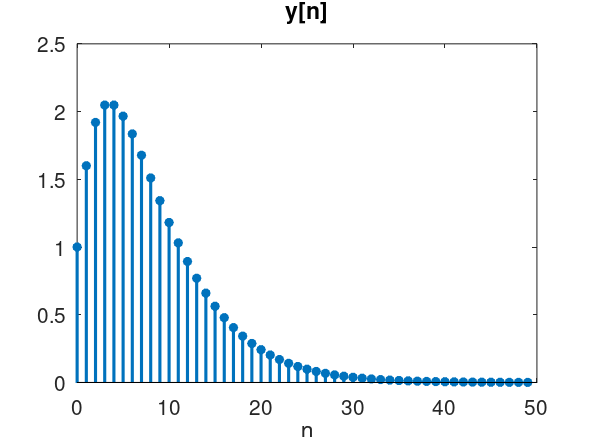
\includegraphics[width=0.7\linewidth]{Imágenes/Figura6}
\end{center}
\end{itemize}
\end{document}